% !TEX root = saveliev_physics_general_course_1.tex
%!TEX TS-program = pdflatex
%!TEX encoding = UTF-8 Unicode


\chapter{NHIỆT ĐỘNG HỌC}\label{chap:12}

\section{Các định luật cơ bản của nhiệt động học}\label{sec:12_1}

Nhiệt học thoạt tiên xuất hiện như một khoa học về các sự biến đổi nhiệt thành công. Tuy nhiên các định luật làm cơ sở cho nhiệt động học có tính chất tổng quát đến mức là hiện nay các phương pháp nhiệt động học đều được áp dụng rất thành công đối với sự nghiên cứu nhiều quá trình vật lý và hoá học và đối với việc nghiên cứu các tính chất của chất và của bức xạ. Như đã được ghi chú trong~\ref{sec:10_1}, khi nghiên cứu các tính chất và các quá trình biến đổi chất, nhiệt động học không đi sâu vào việc khảo sát các hiện tượng bằng cách dựa vào các định luật cơ bản (các nguyên lý) được rút ra từ thực nghiệm. Do nguyên nhân này, các kết luận mà nhiệt động học đạt được có cùng độ tin cậy như là các định luật làm cơ sở cho nhiệt động học. Chính các định luật này là sự khái quát một số lượng khổng lồ các dữ kiện thực nghiệm.

Tạo thành cơ sở của nhiệt động học là hai nguyên lý của nó. Nguyên lý thứ nhất thiết lập các hệ thức định lượng xảy ra khi biến năng lượng từ các dạng này sang các dạng khác. Nguyên lý thứ hai xác định các điều kiện để các biến đổi này có thể xảy ra, nghĩa là xác định các hướng khả dĩ của các quá trình.

Nguyên lý thứ nhất của nhiệt động học khẳng định rằng \textit{nhiệt lượng truyền cho hệ dùng cho sự tăng nội năng của hệ và thực hiện công của hệ lên các vật bên ngoài}:
\begin{equation}\label{eq:12_1}
	Q = U_2 - U_1 + A
\end{equation}

\noindent
hoặc dưới dạng vi phân:
\begin{equation}\label{eq:12_2}
	\derivp{Q} = \deriv{U} + \derivp{A}
\end{equation}

\noindent
[xem~\eqref{eq:10_7} và~\eqref{eq:10_9}].

Đôi khi nguyên lý thứ nhất được diễn đạt như sau: \textit{không thể có được một động cơ vĩnh cửu loại một, nghĩa là một động cơ hoạt động một cách tuần hoàn, thực hiện một công về số lượng lớn hơn năng lượng mà nó thu được từ bên ngoài}.

Mỗi động cơ là một hệ thực hiện nhiều lần quá trình tròn (chu trình) nào đấy. Giả sử trong tiến trình của chu trình, tác nhân (chất khí chẳng hạn) bắt đầu bị dãn đến thể tích $V_2$ và sau đó lại bị nén đến thể tích ban đầu $V_1$ (\fig{12_1}). Để công trong một chu trình lớn hơn không, áp suất (và do đó cả nhiệt độ) trong quá trình dãn phải lớn hơn trong quá trình nén. Muốn vậy trong tiến trình dãn phải truyền nhiệt cho tác nhân sinh công, còn trong tiến trình nén nhiệt được lấy khỏi tác nhân.

\begin{figure}[!htb]
	\begin{center}
		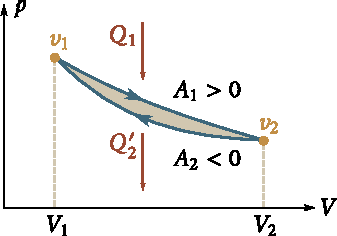
\includegraphics[scale=1.0]{figures/ch_12/fig_12_1.pdf}
		\caption[]{}
		\label{fig:12_1}
	\end{center}
\end{figure}

Sau khi thực hiện một chu trình, tác nhân sinh công lại trở về trạng thái xuất phát. Do đó sự biến đổi nội năng trong một chu trình là bằng không. Nhiệt lượng truyền cho tác nhân sinh công trong một chu trình là bằng $Q_1-Q_2'$, trong đó $Q_1$ là nhiệt do tác nhân sinh công thu được khi dãn, còn $Q_2'$ là nhiệt trả lại khi nén. Công $A$ được thực hiện trong một chu trình bằng diện tích của chu trình (xem~\ref{sec:10_6}). Vậy biểu thức~\eqref{eq:12_1} viết cho một chu trình sẽ có dạng
\begin{equation}\label{eq:12_3}
	A = Q_1 - Q_2'.
\end{equation}

Động cơ hoạt động tuần hoàn thực hiện công do nhiệt nhận được từ bên ngoài được gọi là \textbf{động cơ nhiệt}. Như suy ra từ~\eqn{12_3}, không phải là toàn bộ nhiệt $Q_1$ nhận được từ bên ngoài được dùng để thu công hữu ích. Để động cơ làm việc theo chu trình thì một phần nhiệt bằng $Q_2'$ phải được quay trở lại môi trường bên ngoài và do đó không được dùng trong mục đích của nó (nghĩa là để thực hiện công có ích). Rõ ràng là một động cơ nhiệt biến càng nhiều nhiệt $Q_1$ thu được từ ngoài thành công hữu ích $A$, thì động cơ càng hữu ích. Do đó thông thường người ta đặc trưng cho động cơ nhiệt bằng \textbf{hiệu suất} $\eta$ được xác định như tỷ số công $A$ được thực hiện trong một chu trình với nhiệt $Q_1$ nhận được trong chu trình:
\begin{equation}\label{eq:12_4}
	\eta = \frac{A}{Q_1}.
\end{equation}

\noindent
Nếu chú ý tới hệ thức~\eqn{12_3}, có thể viết biểu thức của hiệu suất dưới dạng
\begin{equation}\label{eq:12_5}
	\eta = \frac{Q_1 - Q_2'}{Q_1}.
\end{equation}

\noindent
Từ định nghĩa của hiệu suất suy ra rằng nó không thể lớn hơn đơn vị.

Nếu quay ngược lại chu trình được biểu diễn trên \fig{12_1} ta thu được chu trình của máy làm lạnh. Một máy như thế trong một chu kỳ sẽ lấy mất của vật có nhiệt độ $T_2$ một nhiệt lượng $Q_2$ và truyền cho vật có nhiệt độ $T_1$ cao hơn một nhiệt lượng $Q_1' $. Công $A'$ phải được thực hiện trên máy trong một chu kỳ. Người ta đặc trưng hiệu suất của máy lạnh bằng hệ số làm lạnh được định nghĩa như tỷ số của nhiệt $Q_2$ được lấy từ vật được làm lạnh với công $A'$ dùng để đưa máy vào hoạt động:
\begin{equation}\label{eq:12_6}
	\beta = \frac{Q_2}{A'} = \frac{Q_2}{Q_1' - Q_2}.
\end{equation}

Nguyên lý thứ hai của nhiệt động học cũng như nguyên lý thứ nhất có thể được trình bày theo một số cách. Một trong các cách trình bày ta đã làm quen ở~\ref{sec:11_11}. Nó được bao hàm trong điều khẳng định là \textit{entropy của một hệ cô lập không thể giảm}:
\begin{equation}\label{eq:12_7}
	\deriv{S} \geqslant 0.
\end{equation}

Nhà vật lý người Đức Rudolf Clausius (1822-1888) đã trình bày nguyên lý thứ hai như sau: \textit{không thể xảy ra các quá trình mà kết quả cuối cùng duy nhất là sự truyền nhiệt từ vật được đốt nóng ít hơn sang vật được đốt nóng nhiều hơn}. Không nên trình bày sự việc như là nguyên lý thứ hai hoàn toàn cấm sự truyền nhiệt từ vật được đốt nóng ít hơn sang vật được đốt nóng nhiều hơn. Trong máy lạnh chính sự truyền nhiệt như vậy được thực hiện. Tuy nhiên sự truyền này không phải là một kết quả duy nhất của quá trình. Nó được kèm theo các biến đổi ở các vật xung quanh liên hệ với sự thực hiện công $A'$ trên hệ.

Ta hãy chứng tỏ rằng một quá trình tưởng tượng được thực hiện trong hệ cô lập, trái ngược với nguyên lý thứ hai ở cách phát biểu của Clausius, sẽ kèm theo sự giảm entropy. Do đó ta chứng minh sự tương đương của cách phát biểu của Clausius và cách diễn đạt thống kê của nguyên lý thứ hai mà theo đó entropy của hệ cô lập không hề giảm.

Bước đầu ta nhận xét như sau. Ta hãy giả thử rằng một vật nào đó trao đổi nhiệt với một vật khác mà ta sẽ gọi là \textbf{bình điều nhiệt}. Giả thử nhiệt dung của bình điều nhiệt là lớn vô cùng. Điều này có nghĩa là khi bình điều nhiệt nhận hoặc toả ra một lượng nhiệt hữu hạn thì nhiệt độ của nó sẽ không biến đổi. Một quá trình diễn biến trong vật kèm theo sự trao đổi nhiệt với bình điều nhiệt có thể là quá trình thuận nghịch chỉ trong trường hợp nếu trong tiến trình của quá trình này nhiệt độ của vật là bằng nhiệt độ của bình điều nhiệt tương ứng. Thật vậy, chẳng hạn nếu vật nhận nhiệt từ bình điều nhiệt với nhiệt độ $T_1$, có nhiệt độ nhỏ hơn $T_1$ thì khi cũng quá trình ấy diễn biến theo hướng ngược lại, vật có thể trả lại cho bình điều nhiệt nhiệt lượng thu được từ nó trong trường hợp nếu nhiệt độ của nó trong mọi trường hợp sẽ không thấp hơn $T_1$. Do đó, trong tiến trình thuận và nghịch của quá trình, nhiệt độ của vật sẽ khác nhau, trong cả hai trường hợp vật đi qua các dãy trạng thái khác nhau (được đặc trưng bằng các nhiệt độ không như nhau) và quá trình được xét sẽ không thuận nghịch.

Vậy quá trình kèm theo sự trao đổi nhiệt chỉ có thể là thuận nghịch trong trường hợp nếu khi nhận nhiệt và trả lại nhiệt cho bình điều nhiệt trong tiến trình ngược, vật sẽ có cùng một nhiệt độ bằng nhiệt độ của bình điều nhiệt. Nói một cách chặt chẽ, khi nhận nhiệt, nhiệt độ của vật phải nhỏ hơn nhiệt độ của bình điều nhiệt (nếu không thì nhiệt không truyền từ bình điều nhiệt tới vật) một lượng vô cùng nhỏ, khi còn nhả nhiệt, nhiệt độ của vật phải cao hơn nhiệt độ của bình điều nhiệt một lượng vô cùng nhỏ.

Do đó quá trình đẳng nhiệt xảy ra ở nhiệt độ của bình điều nhiệt là quá trình thuận nghịch duy nhất có kèm theo sự trao đổi nhiệt với bình điều nhiệt có nhiệt độ không đổi
Ta xét một hệ cô lập gồm hai vật với nhiệt dung $C$ như nhau. Giả thử vật B truyền cho vật A nhiệt lượng $Q$, cho nên nhiệt độ của vật A được nâng lên từ giá trị $\ab{T}{A,$0$}$ đến $\ab{T}{A}$, còn nhiệt độ của vật B giảm từ giá trị $\ab{T}{B,$0$}$ đến $\ab{T}{B}$ ($\ab{T}{B}<\ab{T}{B,$0$}<\ab{T}{A,$0$}<\ab{T}{A}$). Một quá trình như thế mâu thuẫn với nguyên lý thứ hai theo cách diễn đạt của Clausius. Ta hãy tìm độ biến thiên của entropy trong trường hợp này.
Trong tiến trình của quá trình được chỉ ra, sự trao đổi nhiệt xảy ra giữa các vật với các nhiệt độ không như nhau. Theo điều đã nói ở trên, quá trình như thế là không thuận nghịch. Chính công thức~\eqref{eq:11_110} chỉ được áp dụng cho các quá trình thuận nghịch. Để tìm độ biến thiên của entropy trong quá trình không thuận nghịch người ta bắt đầu như sau. Người ta xét một quá trình thuận nghịch nào đó đưa về cùng một trạng thái cuối cùng, giống như quá trình không thuận nghịch đã cho và người ta tính độ biến thiên entropy cho quá trình này theo công thức
\begin{equation}\label{eq:12_8}
	S_2 - S_1 = \int_{1}^{2} \frac{\derivp{Q}}{T}
\end{equation}

\noindent
[xem~\eqn{11_110}].

Căn cứ vào điều đã nói ở trên ta xét một quá trình thuận nghịch mà trong tiến trình của nó vật B nhả nhiệt lượng $Q$ theo các phần $\derivp{Q}$ cho một dãy kế tiếp các bình điều nhiệt với các nhiệt độ có tất cả các giá trị từ $\ab{T}{B,$0$}$ đến $\ab{T}{B}$, còn vật A nhận nhiệt $Q$ theo các phần $\derivp{Q}$ từ một dãy bình điều nhiệt với các nhiệt độ từ $\ab{T}{A,$0$}$ đến $\ab{T}{A}$. Do đó hệ chuyển một cách thuận nghịch từ trạng thái mà các vật có các nhiệt độ $\ab{T}{A,$0$}$ và $\ab{T}{B,$0$}$ sang trạng thái mà các nhiệt độ của các vật bằng $\ab{T}{A}$ và $\ab{T}{B}$. Số gia của entropy trong tiến trình của quá trình này là bằng
\begin{align*}
	\Delta S &= \Delta\ab{S}{A} + \Delta\ab{S}{B} = \int_{\ab{T}{A,$0$}}^{\ab{T}{A}} \frac{C\,\deriv{T}}{T} + \int_{\ab{T}{B,$0$}}^{\ab{T}{B}} \frac{C\,\deriv{T}}{T}\\
	&= C\ln\parenthesis{\frac{\ab{T}{A}}{\ab{T}{A,$0$}}} + C\ln\parenthesis{\frac{\ab{T}{B}}{\ab{T}{B,$0$}}} = C\ln\parenthesis{\frac{\ab{T}{A}\ab{T}{B}}{\ab{T}{A,$0$}\ab{T}{B,$0$}}}.
\end{align*}

\noindent
Nếu để ý rằng $\ab{T}{A}=\ab{T}{A,$0$}+\alpha$ và $\ab{T}{B}=\ab{T}{B,$0$}-\alpha$ ($\alpha=Q/C>0$), ta biểu diễn $\Delta S$ dưới dạng
\begin{equation*}
	\Delta S = C\ln\bracket{\frac{(\ab{T}{A,$0$}+\alpha)(\ab{T}{B,$0$}-\alpha)}{\ab{T}{A,$0$}\ab{T}{B,$0$}}} = C\ln\bracket{1 - \frac{\alpha (\ab{T}{A,$0$} - \ab{T}{B,$0$})}{\ab{T}{A,$0$}\ab{T}{B,$0$}} - \frac{\alpha^2}{\ab{T}{A,$0$}\ab{T}{B,$0$}}}.
\end{equation*}

\noindent
Vì $\ab{T}{A,$0$}>\ab{T}{B,$0$}$ nên biểu thức trong các dấu ngoặc là nhỏ hơn đơn vị, và do đó $\Delta S<0$. Vậy ta đã chứng tỏ rằng trong tiến trình của một quá trình tưởng tượng mâu thuẫn với nguyên lý thứ hai ở cách diễn đạt của Clausius, entropy giảm là điều mâu thuẫn với định luật không giảm của entropy.

Còn một cách diễn đạt nguyên lý thứ hai của nhiệt động học nữa của nhà khoa học người Anh Lord Kelvin (William Thomson, 1824-1907) như sau: \textit{không thể xảy ra các quá trình mà sự lấy một nhiệt lượng xác định từ một vật nào đó và sự biến đổi nhiệt lượng này hoàn toàn ra công là kết quả cuối cùng duy nhất của các quá trình đó}.

Thoạt tiên có thể chứng tỏ rằng cách diễn đạt như thế là mâu thuẫn với, chẳng hạn quá trình dãn khí lý tưởng đẳng nhiệt. Thực vậy, toàn bộ nhiệt lượng do chất khí lý tưởng thu được từ một vật nào đó được biến hoàn toàn ra công. Tuy nhiên sự nhận nhiệt và sự biến đổi nó ra công không phải là kết quả cuối cùng duy nhất của quá trình; ngoài ra, nhờ quá trình này mà sự thay đổi thể tích của chất khí xảy ra.

Trong động cơ nhiệt, sự biến đổi nhiệt ra công nhất thiết kèm theo một quá trình phụ - sự truyền một nhiệt lượng $Q_2'$ nào đó cho vật lạnh hơn, do đó nhiệt lượng $Q_1$ thu được từ vật được nung nóng nhiều hơn không thể bị biến đổi hoàn toàn ra công.

Dễ dàng để tin rằng sự khẳng định chứa đựng trong cách diễn đạt của Kelvin suy ra một cách logic từ sự khẳng định bao hàm trong cách diễn đạt của Clausius. Thật vậy, công có thể được biến đổi hoàn toàn thành nhiệt, chẳng hạn thông qua sự ma sát. Do đó nhờ quá trình bị cách diễn đạt của Kelvin ngăn cấm để biến đổi hoàn toàn nhiệt được lấy từ một vật nào đó ra công và sau đó biến đổi công này, thông qua sự ma sát ra nhiệt truyền cho một vật khác có nhiệt độ cao hơn, ta đã thực hiện được một quá trình không thể xảy ra phù hợp với cách diễn đạt của Clausius.

Khi sử dụng các quá trình bị nguyên lý thứ hai của nhiệt động học ngăn cấm, có thể chế tạo được một động cơ thực hiện công do nhiệt nhận được, chẳng hạn, từ một nguồn năng lượng trên thực tế là không bao giờ cạn là đại dương. Trên thực tế một động cơ như vật là tương đương với một động cơ vĩnh cửu. Do đó nguyên lý thứ hai của nhiệt động học đôi khi được diễn đạt như sau: \textit{không thể có được động cơ vĩnh cửu loại hai, nghĩa là một động cơ hoạt động tuần hoàn, nhận nhiệt từ một bình điều nhiệt và biến đổi hoàn toàn nhiệt này ra công}.

\section{Chu trình Carnot}\label{sec:12_2}

Từ điều đã nói trong mục trước suy ra rằng để động cơ nhiệt làm việc cần có hai bình điều nhiệt. Trong tiến trình của chu trình, động cơ nhận nhiệt lượng $Q_1$ từ một bình điều nhiệt có nhiệt độ $T_1$ cao hơn và được gọi là \textbf{nguồn nóng}; động cơ nhả nhiệt lượng $Q_2'$ cho bình điều nhiệt thứ hai có nhiệt độ $T_2$ thấp hơn và được gọi là \textbf{nguồn lạnh}.

Giả thử rằng nhiệt dung của các bình điều nhiệt là lớn vô cùng. Điều này có nghĩa là các bình điều nhiệt nhận và nhả một lượng nhiệt hữu hạn sẽ không làm thay đổi nhiệt của chúng. Ta hãy tìm hiểu xem tác nhân sinh công của động cơ có thể thực hiện một chu trình thuận nghịch nào trong các điều kiện này. Để ngắn gọn ta sẽ gọi một cách đơn giản các tác nhân sinh công của động cơ là vật.

Rõ ràng là chu trình được xét có thể bao gồm các quá trình mà trong tiến trình của chúng vật sẽ trao đổi nhiệt với các bình điều nhiệt và cả các quá trình không kèm theo sự trao đổi nhiệt với môi trường bên ngoài, nghĩa là các quá trình đoạn nhiệt. Trong mục trước ta đã thành lập được rằng quá trình đẳng nhiệt xảy ra ở nhiệt độ của bình điều nhiệt là quá trình thuận nghịch duy nhất kèm theo sự trao đổi với bình điều nhiệt có nhiệt độ không đổi.

Vậy ta đi tới kết luận là chu trình thuận nghịch do vật thực hiện bắt đầu trao đổi nhiệt với hai bình điều nhiệt có nhiệt dung vô cùng lớp chỉ có thể bao gồm hai quá trình đẳng nhiệt (ở các nhiệt độ của các bình điều nhiệt) và hai quá trình đoạn nhiệt. Một chu trình như vật đầu tiên đã được kỹ sư người Pháp Sadi Carnot (1796-1832) nghiên cứu và mang tên là \textbf{chu trình Carnot}. Ta nhớ rằng chu trình Carnot theo định nghĩa là chu trình thuận nghịch.

Trong quá trình đoạn nhiệt $\derivp{Q}=0$. Do đó theo \eqn{11_110}, trong quá trình đoạn nhiệt thuận nghịch $\deriv{S}=0$, và do đó entropy là không đổi. Trên cơ sở này quá trình đoạn nhiệt thuận nghịch được gọi là \textbf{quá trình đẳng entropy}. Sử dụng thuật ngữ này có thể nói rằng chu trình Carnot bao gồm hai quá trình đẳng nhiệt và hai quá trình đẳng entropy. Trên giản đồ $T$-$S$ chu trình này trông giống như chu trình được trình bày trên \fig{12_2}. Ta chú ý rằng dạng của chu trình Carnot trên giản đồ $T$-$S$ không phụ thuộc vào các tính chất của vật (hoặc của hệ vật) mà đối với các tính chất đó chu trình được biểu diễn.

\begin{figure}[!htb]
	\begin{minipage}[t]{0.5\linewidth}
		\begin{center}
			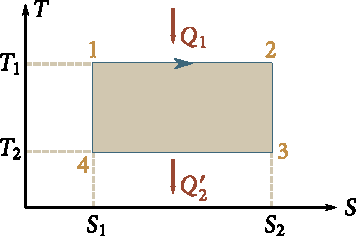
\includegraphics[scale=1.0]{figures/ch_12/fig_12_2.pdf}
			\caption[]{}
			\label{fig:12_2}
		\end{center}
	\end{minipage}
	\hspace{-0.05cm}
	\begin{minipage}[t]{0.5\linewidth}
		\begin{center}
			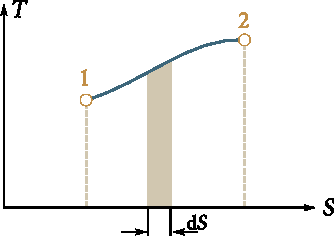
\includegraphics[scale=1.0]{figures/ch_12/fig_12_3.pdf}
			\caption[]{}
			\label{fig:12_3}
		\end{center}
	\end{minipage}
\end{figure}

Trên hình~\ref{fig:12_3} người ta biểu diễn một quá trình nào đó chuyển hệ từ trạng thái $1$ sang trạng thái $2$. Theo~\eqn{11_110} nhiệt lượng nguyên tố $\derivp{Q}$ do hệ nhận được có thể được biểu diễn dưới dạng $T\,\deriv{S}$. Do đó diện tích của dải được gạch gạch trên \fig{12_3} là bằng $\derivp{Q}$, còn diện tích của hình được giới hạn bởi đường cong $1$-$2$ cho nhiệt lượng do hệ nhận được trong tiến trình của quá trình. Một cách tương tự, diện tích của hình được giới hạn bởi đường con biểu diễn quá trình trên giản đồ $p$-$V$ cho công do hệ thực hiện trong tiến trình của quá trình (xem \fig{10_4}).

Theo điều đã được nói, diện tích của chu trình trên \fig{12_2} cho nhiệt lượng do hệ nhận được trong tiến trình của chu trình (nó bằng $Q_1-Q_2'$). Một cách tương tự, diện tích của chu trình trên giản đồ $p$-$V$ cho công do hệ thực hiện trong một chu trình (xem \fig{10_5}).

Có thể tính nhiệt lượng do hệ nhận được trong tiến trình của một quá trình thuận nghịch tuỳ ý theo công thức
\begin{equation}\label{eq:12_9}
	Q = \int_{1}^{2} T\,\deriv{S}
\end{equation}

\noindent
[so sánh với~\eqn{10_12}].

Ta tìm hiệu suất của chu trình Carnot. Sau khi thực hiện một chu trình, hệ trở về trạng thái ban đầu. Do đó sự biến đổi hoàn toàn của entropy trong một chu trình là bằng không. Trên đoạn $1$-$2$ (xem \fig{12_2}), hệ nhận được một nhiệt lượng $Q_1$ từ bình điều nhiệt có nhiệt độ $T_1$. Số gia của entropy trên đoạn này là bằng
\begin{equation*}
	\Delta S_{12} = \int_{1}^{2} \frac{\derivp{Q}}{T_1} = \frac{1}{T_1} \int_{1}^{2} \derivp{Q} = \frac{Q_1}{T_1}.
\end{equation*}

\noindent
Trên đoạn $3$-$4$ hệ nhả nhiệt lượng $Q_2'$ cho bình điều nhiệt có nhiệt độ $T_2$. Việc lấy đi ở vật nhiệt lượng $Q_2'$ tương đương với việc truyền cho vật nhiệt lượng $-Q_2'$. Do đó số gia của entropy trên đoạn $3$-$4$ là bằng
\begin{equation*}
	\Delta S_{34} = \int_{3}^{4} \frac{\derivp{Q}}{T_2} = \frac{1}{T_2} \int_{3}^{4} \derivp{Q} = -\frac{Q_2'}{T_2}.
\end{equation*}

\noindent
Trên các đoạn $2$-$3$ và $4$-$1$ entropy là không đổi. Vậy số gia toàn phần của entropy trong một chu kỳ sẽ bằng
\begin{equation}\label{eq:12_10}
	\Delta S_{12} + \Delta S_{34} = \frac{Q_1}{T_1} - \frac{Q_2'}{T_2} = 0.
\end{equation}

\noindent
Từ \eqn{12_10} suy ra rằng
\begin{equation}\label{eq:12_11}
	\frac{Q_1}{T_1} = \frac{Q_2'}{T_2}.
\end{equation}

Có thể biểu diễn biểu thức~\eqref{eq:12_5} đối với hiệu suất của máy nhiệt dưới dạng
\begin{equation}\label{eq:12_12}
	\eta = \frac{Q_1-Q_2'}{Q_1} = 1 - \frac{Q_2'}{Q_1}.
\end{equation}

\noindent
Thay thế trong biểu thức này tỷ số $Q_2'/Q_1$ ứng với~\eqn{12_11} ta thu được là
\begin{equation}\label{eq:12_13}
	\eta = 1 - \frac{T_2}{T_1} = \frac{T_1 - T_2}{T_1}.
\end{equation}

Khi rút ra công thức~\eqn{12_13} ta đã không nêu ra các giả thuyết nào về các tính chất của tác nhân sinh công và cơ cấu của động cơ nhiệt. Do đó ta đi tới điều khẳng định là \textit{hiệu suất của tất cả các động cơ thuận nghịch làm việc trong những điều kiện như nhau (nghĩa là với cùng một nhiệt độ của nguồn nóng và nguồn lạnh) đều giống nhau và được xác định chỉ bởi nhiệt độ của nguồn nóng và nguồn lạnh}. Điều khẳng định này mang tên là \textbf{định lý Carnot}.

Ta xét một động cơ không thuận nghịch làm việc với cùng các nguồn nóng và nguồn lạnh giống như các nguồn của một động cơ thuận nghịch làm việc theo chu trình Carnot. Giả sử sau mỗi chu trình, động cơ trở về trạng thái ban đầu mà ta sẽ xem là trạng thái cân bằng. Vì entropy là một hàm của trạng thái nên số gia của nó trong một chu trình phải bằng không:
\begin{equation*}
	\oint \deriv{S} = 0.
\end{equation*}

Vì các quá trình tạo thành chu trình là không thuận nghịch nên đối với mỗi quá trình nguyên tố có bất đẳng thức $\deriv{S}>\derivp{Q}/T$ [xem ~\eqref{eq:11_111}). Do đó, từ điều kiện bằng không của số gia toàn phần của entropy trong một chu trình, suy ra rằng
\begin{equation*}
	0 = \oint \deriv{S} > \oint \frac{\derivp{Q}}{T}
\end{equation*}

\noindent
từ đó
\begin{equation}\label{eq:12_14}
	\oint \frac{\derivp{Q}}{T} < 0.
\end{equation}

\noindent
Ta hãy chia tích phân~\eqref{eq:12_14} thành bốn số hạng:
\begin{equation}\label{eq:12_15}
	\oint \frac{\derivp{Q}}{T} = \int_{T_1} \frac{\derivp{Q}}{T} + \int_{\text{Ad}1} \frac{\derivp{Q}}{T} + \int_{T_2} \frac{\derivp{Q}}{T} + \int_{\text{Ad}2} \frac{\derivp{Q}}{T} < 0.
\end{equation}

\noindent
Số hạng thứ nhất ứng với quá trình nhận nhiệt lượng $Q_1$ từ bình điều nhiệt với nhiệt độ $T_1$ (nhiệt lượng đó không nhất thiết trùng với nhiệt lượng $Q_1$ mà động cơ thuận nghịch nhận trong một chu trình). Số hạng thứ hai ứng với phần đoạn nhiệt của chu trình. Số hạng thứ ba ứng với quá trình truyền nhiệt lượng $Q_2'$ cho bình điều nhiệt với nhiệt độ $T_2$ (nhiệt lượng đó không nhất thiết trùng với nhiệt lượng $Q_2'$ mà động cơ thuận nghịch nhả trong một chu trình). Cuối cùng số hạng thứ tư ứng với phần đoạn nhiệt chu trình. Trên các thành phần đoạn nhiệt $\derivp{Q}=0$, vì vậy các tích phân tương ứng bằng không. Tích phân ứng với phần $T_1$ bằng $Q_1/T_1$ (ta nhớ tằng trong trường hợp quá trình không thuạn nghịch, ở mẫu số của tỷ số $\derivp{Q}/T$ là nhiệt độ của bình điều nhiệt mà vật đã cho nhạ anhiệt lượng $\derivp{Q}$). Tích phân ứng với phần $T_2$ bằng $-Q_2'/T_2$. Như vậy, ta đi tới bất đẳng thức
\begin{equation}\label{eq:12_16}
	\frac{Q_1}{T_1} - \frac{Q_2'}{T_2}  < 0.
\end{equation}

\noindent
Từ ~\eqref{eq:12_16}, ta thu được
\begin{equation*}
	\frac{Q_2'}{Q_1} > \frac{T_2}{T_1}
\end{equation*}

\noindent
và do đó
\begin{equation}\label{eq:12_17}
	\eta = 1 - \frac{Q_2'}{Q_1} < 1 - \frac{T_2}{T_1} = \frac{T_1 - T_2}{T_1}.
\end{equation}

\noindent
Kết quả thu được có nghĩa là hiệu suất của động cơ không thuận nghịch luôn luôn nhỏ hơn hiệu suất của động cơ thuận nghịch làm việc trong cùng các điều kiện.

\begin{figure}[!htb]
	\begin{center}
		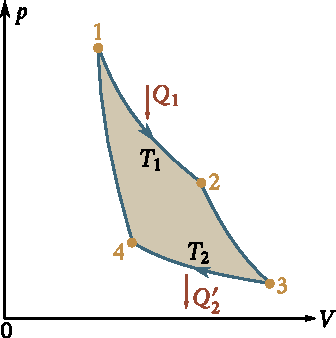
\includegraphics[scale=1.0]{figures/ch_12/fig_12_4.pdf}
		\caption[]{}
		\label{fig:12_4}
	\end{center}
	\vspace{-0.8cm}
\end{figure}

Dạng của chu trình Carnot trên giản đồ $p$-$V$ phụ thuộc vào các tính chất của chất thực hiện chu trình. Đối với khí lý tưởng chu trình trông giống như chu trình được biểu diễn trên \fig{12_4}. Có thể tính hiệu suất của chu trình Carnot đối với khí lý tưởng mà không cần tìm số gia của entropy.

Trong quá trình đẳng nhiệt nội năng của khí lý tưởng vẫn không đổi. Do đó nhiệt lượng $Q_1$ mà chất khí nhận được là bằng công $A_{12}$ do chất khí thực hiện khi chuyển từ trạng thái $1$ sang trạng thái $2$ (\fig{12_4}). Theo \eqn{10_60} công này bằng
\begin{equation}\label{eq:12_18}
	Q_1 = A_{12} = \frac{m}{M}RT_1 \ln\parenthesis{\frac{V_2}{V_1}}
\end{equation}

\noindent
trong đó $m$ là một khối lượng của khí lý tưởng trong máy. Nhiệt lượng $Q_2'$ trao cho nguồn lạnh là bằng công $A_{34}'$ được tiêu tốn cho sự nén khí khi chuyển nó từ trạng thái $3$ sang trạng thái $4$. Công này bằng
\begin{equation}\label{eq:12_19}
	Q_2' = A_{34}' = \frac{m}{M}RT_2 \ln\parenthesis{\frac{V_3}{V_4}}.
\end{equation}

Để chu trình được khép kín các trạng thái $1$ và $4$ phải nằm trên cùng một quá trình đoạn nhiệt. Từ đó suy ra điều kiện
\begin{equation}\label{eq:12_20}
	T_1 V_1^{\gamma-1} = T_2 V_2^{\gamma-1}.
\end{equation}

\noindent
[xem phương trình đoạn nhiệt ~\eqref{eq:10_41}]. Một cách tương tự, vì các trạng thái $2$ và $3$ đều nằm trên cùng một quá trình đoạn nhiệt nên điều kiện
\begin{equation}\label{eq:12_21}
	T_3 V_3^{\gamma-1} = T_4 V_4^{\gamma-1}.
\end{equation}

\noindent
được nghiệm đúng. Chia \eqn{12_21} cho~\eqref{eq:12_20}, ta đi tới điều kiện về sự đóng kín của chu trình:
\begin{equation}\label{eq:12_22}
	\frac{V_2}{V_1} = \frac{V_3}{V_4}.
\end{equation}

Bây giờ ta thay thế~\eqref{eq:12_18} và~\eqref{eq:12_19}, vào \eqn{12_5} đối với hiệu suất:
\begin{equation*}
	\eta = \frac{\dfrac{m}{M}RT_1\ln\parenthesis{\dfrac{V_2}{V_1}} - \dfrac{m}{M}RT_2\ln\parenthesis{\dfrac{V_3}{V_4}}}{\dfrac{m}{M}RT_1\ln\parenthesis{\dfrac{V_2}{V_1}}}.
\end{equation*}

\noindent
Cuối cùng, nếu để ý tới điều kiện~\eqref{eq:12_22} ta thu được biểu thức
\begin{equation*}
	\eta = \frac{T_1 - T_2}{T_1}
\end{equation*}

\noindent
trùng với \eqn{12_13}.

\section{Thang nhiệt độ nhiệt động học}\label{sec:12_3}

Định lý về sự không phụ thuộc của hiệu suất các động cơ thuận nghịch vào các tính chất của tác nhân sinh công đã được chính minh trong mục trước cho phép thiết lập thang nhiệt độ không phụ thuộc vào việc chọn vật nhiệt biểu. Căn cứ vào định lý đã nêu, đại lượng
\begin{equation*}
	\eta = \frac{Q_1 - Q_2'}{Q_1} = 1 - \frac{Q_2'}{Q_1}
\end{equation*}

\noindent
và do đó cả tỷ số $Q_2'/Q_1$ đối với chu trình Carnot đều chỉ phụ thuộc vào các nhiệt độ của nguồn nóng và nguồn lạnh. Ký hiệu các độ lớn của các nhiệt độ này theo một thang nào đó trong khi ta chưa biết rằng, $\theta_1$ và $\theta_2$, thì có thể viết được là
\begin{equation}\label{eq:12_23}
	\frac{Q_2'}{Q_1} = f(\theta_1,\theta_2)
\end{equation}

\noindent
trong đó $f(\theta_1,\theta_2)$ là một hàm phổ biến (nghĩa là giống nhau đối với mọi chu trình Carnot) của các nhiệt độ của nguồn nóng và nguồn lạnh. Hệ thức~\eqref{eq:12_23} cho khả năng xác định nhiệt độ của các vật qua nhiệt lượng nhận vào và nhả ra trong các chu trình Carnot.

Ta chứng minh rằng hàm~\eqref{eq:12_23} có tính chất sau đây:
\begin{equation}\label{eq:12_24}
	f(\theta_1,\theta_2) = \frac{\Theta(\theta_2)}{\Theta(\theta_1)}
\end{equation}

\noindent
trong đó $\Theta(\theta)$ lại là hàm phổ biến của nhiệt độ. Ta xét hai động cơ thuận nghịch M$_1$ and M$_2$ (\fig{12_5}) mà nguồn lạnh của máy này lại đồng thời là nguồn nóng của máy kia. Ta giả thiết rằng máy thứ hai lấy từ bình điều nhiệt có nhiệt độ $\theta_1$ cùng một nhiệt lượng mà máy thứ nhất nhả cho nó.

\begin{figure}[!htb]
	\begin{center}
		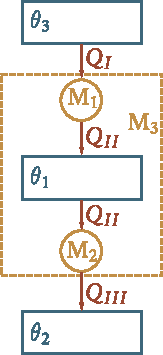
\includegraphics[scale=1.0]{figures/ch_12/fig_12_5.pdf}
		\caption[]{}
		\label{fig:12_5}
	\end{center}
	\vspace{-0.8cm}
\end{figure}

Đối với máy M$_1$: $Q_1=Q_I$, $Q_2'=Q_{II}$. Do đó \eqn{12_23} đối với máy này có dạng
\begin{equation}\label{eq:12_25}
	\frac{Q_{II}}{Q_I} = f(\theta_3,\theta_1).
\end{equation}

\noindent
Đối với máy M$_2$: $Q_1=Q_{II}$, $Q_2'=Q_{III}$. Do đó theo \eqn{12_23}
\begin{equation}\label{eq:12_26}
	\frac{Q_{III}}{Q_{II}} = f(\theta_1,\theta_2).
\end{equation}

\noindent
Nếu coi các máy M$_1$ và M$_2$ và cả bình điều nhiệt có nhiệt độ $\theta_1$ như một máy thuận nghịch duy nhất nhận nhiệt lượng $Q_I$ từ nguồn nóng có nhiệt độ $\theta_3$ và nhả nhiệt lượng $Q_{III}$ cho nguồn lạnh có nhiệt độ $\theta_2$ thì có thể viết:
\begin{equation}\label{eq:12_27}
	\frac{Q_{III}}{Q_{I}} = f(\theta_3,\theta_2).
\end{equation}

Chia \eqn{12_27} cho~\eqref{eq:12_25} ta được
\begin{equation*}
	\frac{Q_{III}}{Q_{II}} = \frac{f(\theta_3,\theta_2)}{f(\theta_3,\theta_1)}.
\end{equation*}

\noindent
So sánh biểu thức này với \eqn{12_26} đưa tới hệ thức
\begin{equation}\label{eq:12_28}
	f(\theta_1,\theta_2) = \frac{f(\theta_3,\theta_2)}{f(\theta_3,\theta_1)}.
\end{equation}

\noindent
Hệ thức này liên hệ với các nhiệt độ $\theta_1$ và $\theta_2$ của hai vật với nhau, thêm vào đó nhiệt độ $\theta_3$ của vật thứ ba cũng có mặt trong hệ thức đó. Nếu qui ước một cách dứt khoát về việc chọn vật này, nghĩa là làm cho $\theta_3$ không thay đổi thì ta sẽ chuyển hàm $f(\theta_3,\theta)$ ở tử số và mẫu số của công thức \eqn{12_28} tới hàm một biến $\theta$. Ký hiệu hàm này qua $\Theta(\theta)$ ta đi tới công thức \eqn{12_24}.

Hàm $\Theta(\theta)$ chỉ phụ thuộc vào nhiệt độ. Do đó có thể sử dụng các giá trị của nó để đặc trưng nhiệt độ của vật tương ứng, nghĩa là giả định nhiệt độ của vật bằng $\Theta$ trong đó $\Theta=\Theta(\theta)$. Khi đó biểu thức~\eqref{eq:12_23} có dạng sau:
\begin{equation}\label{eq:12_29}
	\frac{Q_2'}{Q_1} = \frac{\Theta_2}{\Theta_1}.
\end{equation}

\noindent
Hệ thức~\eqref{eq:12_29} làm cơ sở cho cái gọi là \textbf{thang nhiệt độ nhiệt động học}. Sự ưu việt của thang này là ở chỗ nó không phụ thuộc vào việc chọn vật (tác nhân sinh công trong chu trình Carnot), được dùng để đo nhiệt độ.

Theo \eqn{12_29} để so sánh các nhiệt độ của hai vật cần thực hiện một chu trình Carnot, bằng cách sử dụng các vật này để làm nguồn nóng và nguồn lạnh. Tỷ số nhiệt lượng nhả cho một vật là ``nguồn lạnh'' với nhiệt lượng lấy từ một vật là ``nguồn nóng'' cho tỷ số các nhiệt độ của các vật được xét. Để xác định đơn trị trị số $\Theta$ cần quy ước về cách chọn đơn vị nhiệt độ, nghĩa là độ. Một phần trăm hiệu các nhiệt độ của nước sôi ở áp suất khí quyển và của nước đá đang tan được lấy làm một độ tuyệt đối. Vậy một độ của thang nhiệt động học tuyệt đối là bằng một độ của thang khí lý tưởng.

Dễ dàng thiết lập được rằng thang nhiệt độ nhiệt động học trùng với thang khí lý tưởng. Thực vậy, theo \eqn{12_11}
\begin{equation}\label{eq:12_30}
	\frac{Q_2'}{Q_1} = \frac{T_2}{T_1}.
\end{equation}

\noindent
So sánh ~\eqref{eq:12_29} với~\eqref{eq:12_30} ta thu được là
\begin{equation*}
	\frac{\Theta_2}{\Theta_1} = \frac{T_2}{T_1}.
\end{equation*}

\noindent
Do đó, $\Theta$ tỷ lệ với $T$ và vì sự chia độ của hai thang là như nhau nên $\Theta=T$.

\section{Các ví dụ về cách tính Entropy}\label{sec:12_4}

Entropy là một hàm của trạng thái. Vì vậy nó phải phụ thuộc vào tham số xác định trạng thái của hệ. Chẳng hạn, entropy có thể được xác định như hàm của $p$ và $T$ hoặc như hàm của $V$ và $T$, v.v... Giả sử rằng một vật nào đó được đốt nóng ở áp suất không đổi $p$ từ không độ tuyệt đối đến nhiệt độ $T$, hơn nữa quá trình đốt nóng xảy ra là thuận nghịch. Khi đó theo ~\eqref{eq:11_110} và~\eqref{eq:10_24} entropy của vật ở áp suất $p$ và nhiệt độ $T$ được xác định bởi biểu thức
\begin{equation}\label{eq:12_31}
	S(p,T) = \int_{0}^{T} \frac{C_p(T)\,\deriv{T}}{T}
\end{equation}

\noindent
trong đó $C_p(T)$ là nhiệt dung của vật ở áp suất không đổi, mà nó là một hàm của nhiệt độ. Một cách tương tự, entropy như hàm của thể tích $V$ và nhiệt độ $T$ có thể được biểu diễn dưới dạng
\begin{equation}\label{eq:12_32}
	S(V,T) = \int_{0}^{T} \frac{C_V(T)\,\deriv{T}}{T}
\end{equation}

\noindent
trong đó $C_V$ là nhiệt dung của vật ở thể tích không đổi.

Từ các công thức ~\eqref{eq:12_31} và~\eqref{eq:12_32} suy ra rằng các nhiệt dung $C_p$ và $C_V$ (cũng như nhiệt dung ở mọi quá trình khác) triệt tiêu ở không độ tuyệt đối. Thật vậy, nếu nhiệt dung không tiến tới không kh $T$ tiến tới 0 thì hàm dưới dấu tích phân tăng vô hạn, do đó tích phân là phân kỳ (tức là trở thành vô hạn).

\textbf{1. Entropy của khí lý tưởng}. Trong ~\ref{sec:11_11} đã tìm được biểu thức đối với entropy của chất khí lý tưởng đơn nguyên tử (tức là chất khí có $C_V=3R/2$). Bây giờ sử dụng \eqn{11_110} ta thu được biểu thức đối với entropy của chất khí với các phân tử tuỳ ý. Vì entropy là cộng tính nên chỉ cần tìm giá trị $\ab{S}{m}$ của nó đối với một mol khí. Entropy của một khối lượng khí tuỳ ý sẽ bằng $S=(m/M)\ab{S}{m}$.

Ta sẽ đặc trưng trạng thái của chất bởi các tham số $V$ và $T$, tuy nhiên ta sẽ không coi quá trình đang xét là quá trình đẳng tích. Theo định lý Nernst và công thức \eqn{11_110}
\begin{equation}\label{eq:12_33}
	\ab{S}{m}(V,T) = \int_{0}^{(V,T)} \frac{\derivp{Q}}{T}
\end{equation}

\noindent
trong đó trạng thái của chất khí được ký hiệu bằng $(V, T)$ (ta chú ý là V của một mol). Việc lấy tích phân được thực hiện theo một quá trình thuận nghịch tuỳ ý chuyển chất từ trạng thái ở không độ tuyệt đối sang trạng thái được đặc trưng bằng thể tích $V$ và nhiệt độ $T$.

Ta hãy lấy thể tích $V_0$ và nhiệt độ $T_0$ mà trong đó chất rõ ràng là khí lý tưởng, và chia tích phân trong công thức \eqn{12_33} thành hai:
\begin{equation}\label{eq:12_34}
	\ab{S}{m}(V,T) = \int_{0}^{(V_0,T_0)} \frac{\derivp{Q}}{T} + \int_{(V_0,T_0)}^{(V,T)} \frac{\derivp{Q}}{T}.
\end{equation}

\noindent
Tích phân thứ nhất là một số nào đó mà ta ký hiệu nó qua $S(V_0,T_0)$. Tích phân thứ hai là hàm của $V$ và $T$. Để tìm được dạng của hàm này ta biểu diễn $\derivp{Q}$ dưới dạng $\derivp{Q}=C_V\,\deriv{T}+p\,\deriv{V}$ (trong khoảng lấy tích phân chất thể hiện như một chất khí lý tưởng). Chia $\derivp{Q}$ cho $T$ và dựa vào phương trình trạng thái thay thế $R/V$ qua $p/T$ ta thu được:
\begin{equation*}
	\int_{(V_0,T_0)}^{(V,T)} \frac{\derivp{Q}}{T} = \int_{T_0}^{T} \frac{C_V\,\deriv{T}}{T} + \int_{V_0}^{V} \frac{R\,\deriv{V}}{V} = C_V\ln\parenthesis{\frac{T}{T_0}} + R\ln\parenthesis{\frac{V}{V_0}}.
\end{equation*}

\noindent
Vậy công thức \eqn{12_34} có dạng
\begin{equation}\label{eq:12_35}
	\ab{S}{m}(V,T) = S(V_0,T_0) + C_V\ln\parenthesis{\frac{T}{T_0}} + R\ln\parenthesis{\frac{V}{V_0}}.
\end{equation}

\noindent
Ta biến đổi công thức này như sau\footnote{Không nên nghi ngại rằng dưới dấu loga lại có đại lượng có thứ nguyên. Trong các biểu thức chứa $\ln{f}$ luôn luôn có số hạng chứa $\ln{f_0}$ ($f_0$ là một hằng số) với dấu sao cho $\ln{f}$ và $\ln{f_0}$ có thể được hợp nhất vào một số hạng có dạng $\ln(f/f_0)$.}
\begin{equation}\label{eq:12_36}
	\ab{S}{m} = C_V\ln{T} + R\ln{V} + S_0
\end{equation}

\noindent
trong đó $S_0$ là một hằng số bằng $S(V_0,T_0)-\ln{T_0}-\ln{V_0}$.

Ta chú ý rằng hoặc các đạo hàm của entropy theo các tham số trạng thái, hoặc sự biến đổi của entropy thường sẽ tham gia vào các hệ thức mà trên thực tế ta đã từng gặp chúng. Trong các trường hợp này việc tìm giá trị của hằng số cộng trong biểu thức đối với entropy là không cần thiết.

Công thức~\eqref{eq:12_36} cho biểu thức của entropy của một mol khí lý tưởng theo các biến số $V$ và $T$. Nhờ phương trình trạng thái có thể chuyển tới các biểu thức của entropy theo các biến số khác. Thay thế $V=RT/p$ vào \eqn{12_36} ta thu được công thức
\begin{equation*}
	\ab{S}{m} = C_V\ln{T} + R\ln{R} + R\ln{T} - R\ln{p} + S_0.
\end{equation*}

\noindent
Để ý rằng đối với khí lý tưởng $C_V+R=C_p$ có thể viết:
\begin{equation}\label{eq:12_37}
	\ab{S}{m} = C_p\ln{T} + R\ln{p} + S_0'
\end{equation}

\noindent
trong đó $S_0'=S_0+R\ln{R}$.

Cuối cùng, thay $T$ bằng $pV/R$ vào \eqn{12_36} ta đi tới công thức
\begin{equation}\label{eq:12_38}
	\ab{S}{m} = C_V\ln{p} + C_p\ln{V} + S_0''
\end{equation}

\noindent
trong đó $S_0''=S_0-V_C\ln{R}$.

\textbf{2. Entropy của nước.} Các thay đổi của nhiệt dung của nước trong khoảng từ \SI{0}{\degreeCelsius} đến \SI{100}{\degreeCelsius} không vượt quá 1\%. Do đó trong khoảng nhiệt độ được chỉ ra có thể coi nhiệt dung riêng của nước là một hằng số bằng $c=\SI{4.2}{\kilo\joule\per\kilo\gram\per\kelvin}$. Một các tương ứng, ta ký hiệu $s(273)$ là entropy riêng của nước lỏng ở \SI{0}{\degreeCelsius} còn $s(T)$ là entropy riêng của nước ở nhiệt độ $T$ ($273<T<373$), ta có thể viết được là
\begin{equation*}
	s(T) - s(273) \int_{273}^{T} \frac{c\,\deriv{T}}{T} = c\ln\parenthesis{\frac{T}{273}}
\end{equation*}

\noindent
từ đó
\begin{equation}\label{eq:12_39}
	s(T) = c\ln{T} + [s(273) - c\ln(273)] = c\ln{T} + \text{constant}.
\end{equation}

\textbf{3. Sự thay đổi của entropy khi nóng chảy}. Nếu áp suất không thay đổi thì sự nóng chảy xảy ra ờ nhiệt độ không đổi. Một cách tương ứng, số gia của entropy riêng là bằng
\begin{equation}\label{eq:12_40}
	\Delta s = \int_{\text{sol}}^{\text{liq}} \frac{\derivp{Q}}{\ab{T}{f}} = \frac{1}{\ab{T}{f}} \int_{\text{sol}}^{\text{liq}} \derivp{Q} = \frac{\ab{L}{f}}{\ab{T}{f}}
\end{equation}

\noindent
trong đó $\ab{L}{f}$ là nhiệt nóng chảy riêng. Khi chất đông đặc lại entropy riêng bị giảm cùng một lượng như vậy.

Công thức đối với số gia của entropy riêng khi bay hơi khác với \eqn{12_40} chỉ ở chỗ là thay cho nhiệt và nhiệt độ nóng chảy là nhiệt bay hơi và nhiệt độ sôi tham gia vào \eqn{12_40}

\section{Một số ứng dụng của entropy}\label{sec:12_5}

Ta hãy lấy thể tích $V$ và nhiệt độ $T$ làm các tham số độc lập đặc trưng trạng thái của một chất nào đó. Khi đó nội năng của chất sẽ là hàm của các tham số đó: $U=U(V, T)$. Trong trường hợp này biểu thức của nguyên lý thứ nhất của nhiệt động học có dạng\footnote{Vi phân toàn phần của hàm $f(x,y)$ của các biến số $x$ và $y$ được xác định bằng biểu thức $\deriv{f}=\diffinpartial{f}{x}\,\deriv{x}+\diffinpartial{f}{y}\,\deriv{y}$. Biểu thức này cho số gia của hàm $f(x,y)$ trong trường hợp mà các biến số $x$ và $y$ nhận được các số gia $\deriv{x}$ và $\deriv{y}$ [xem \eqn{3_33}].}
\begin{equation}\label{eq:12_41}
	\derivp{Q} = \parenthesis{\diffpartial{U}{T}}_V\,\deriv{T} + \parenthesis{\diffpartial{U}{V}}_T\,\deriv{V} + p\,\deriv{V}.
\end{equation}

\noindent
Trong nhiệt động học ta thường thêm vào các đạo hàm riêng của các hàm số theo các tham số trạng thái một số chỉ ra tham số nào được giả thiết là không đổi trong phép lấy vi phân. Điều này là cần thiết vì, chẳng hạn, có thể xét đạo hàm riêng của $U$ theo $T$ với điều kiện là $p$ = constant. Đạo hàm này được ký hiệu bằng $(\diffinpartial{U}{T})_p$ và, nói chung, có giá trị khác so với $(\diffinpartial{U}{T})_V$.

Chia biểu thức \eqn{12_41} cho $T$ ta được số gia của entropy:
\begin{equation}\label{eq:12_42}
	\deriv{S} = \bracket{\frac{1}{T} \parenthesis{\diffpartial{U}{T}}_V} \, \deriv{T} + \bracet{\frac{1}{T} \bracket{\parenthesis{\diffpartial{U}{V}}_T + p}}\,\deriv{V}.
\end{equation}

\noindent
Coi entropy như một hàm của các tham số $V$ và $T$, có thể biểu diễn số gia của entropy dưới dạng
\begin{equation*}
	\deriv{S} = \parenthesis{\diffpartial{S}{T}}_V\,\deriv{T} + \parenthesis{\diffpartial{S}{V}}_T\,\deriv{V}.
\end{equation*}

\noindent
So sánh với \eqn{12_42} ta được
\begin{equation}\label{eq:12_43}
	\parenthesis{\diffpartial{S}{T}}_V = \frac{1}{T} \parenthesis{\diffpartial{U}{T}}_V,\quad \parenthesis{\diffpartial{S}{V}}_T = \frac{1}{T} \bracket{\parenthesis{\diffpartial{U}{V}}_T + p}.
\end{equation}

Các đạo hàm riêng hỗn hợp của một hàm $f(x, y)$ nào đó thoả mãn điều kiện
\begin{equation*}
	\frac{\uppartial^2f}{\uppartial x\,\uppartial y} = \frac{\uppartial^2f}{\uppartial y\,\uppartial x}.
\end{equation*}

\noindent
Căn cứ vào điều này
\begin{equation*}
	\frac{\uppartial}{\uppartial V} \parenthesis{\diffpartial{S}{T}}_V = \frac{\uppartial}{\uppartial T} \parenthesis{\diffpartial{S}{V}}_T.
\end{equation*}

\noindent
Việc thay thế biểu thức~\eqref{eq:12_43} vào đẳng thức này sẽ dẫn tới hệ thức
\begin{equation*}
	\frac{\uppartial}{\uppartial V} \bracket{\frac{1}{T} \parenthesis{\diffpartial{U}{T}}_V} = \frac{\uppartial}{\uppartial T} \bracet{\frac{1}{T} \bracket{\parenthesis{\diffpartial{U}{V}}_T + p}}.
\end{equation*}

\noindent
Thực hiện phép lấy vi phân, ta được
\begin{equation*}
	\frac{1}{T}\frac{\uppartial^2U}{\uppartial V\,\uppartial T} = -\frac{1}{T^2} \bracket{\parenthesis{\diffpartial{U}{V}}_T + p} + \frac{1}{T} \bracket{\frac{\uppartial^2U}{\uppartial T\,\uppartial V} + \parenthesis{\diffpartial{p}{T}}_V}.
\end{equation*}

\noindent
Chú ý rằng $\uppartial^2U/\uppartial V\,\uppartial T$, ta đi đến công thức
\begin{equation}\label{eq:12_44}
	\parenthesis{\diffpartial{U}{V}}_T = T \parenthesis{\diffpartial{p}{T}}_V - p.
\end{equation}

Công thức \eqn{12_44} đặc trưng cho sự phụ thuộc của nội năng vào thể tích. Ta áp dụng nó để tìm nội năng của các chất khí lý tưởng và khí van der Waals.

Đối với khí lý tưởng $p=RT/V$. Do đó $(\diffinpartial{p}{T})_V=R/V$. Thay thế giá trị này vào \eqn{12_44} ta được
\begin{equation*}
	\parenthesis{\diffpartial{U}{V}}_T = T\frac{R}{V} - p = 0.
\end{equation*}

\noindent
Kết quả thu được có nghĩa là nội năng của khí lý tưởng không phụ thuộc vào thể tích. Trong~\ref{sec:10_9} ta đã đi tới cùng một kết luận bằng cách dựa trên giả thuyết về sự không có mặt các tương tác giữa các phân tử.

Từ phương trình trạng thái của khí van der Waals [xem \eqn{10_62}] suy ra rằng
\begin{equation}\label{eq:12_45}
	p = \frac{RT}{(V - b)} - \frac{a}{V^2}.
\end{equation}

\noindent
Từ đó
\begin{equation*}
	\parenthesis{\diffpartial{p}{T}}_V = \frac{R}{(V-b)}.
\end{equation*}

\noindent
Thay thế biểu thức này vào công thức~\eqref{eq:12_44} ta được
\begin{equation*}
	\parenthesis{\diffpartial{U}{V}}_T = \frac{RT}{(V - b)} - p = \frac{a}{V^2}.
\end{equation*}

\noindent
[xem \eqn{12_45}]. Lấy tích phân theo $V$ ta tìm được
\begin{equation*}
	U = -\frac{a}{V} + f(T).
\end{equation*}

\noindent
Có thể thiết lập được dạng của hàm $f(T)$ bằng cách sử dụng điều là khi $V$ tiến tới vô cùng, biểu thức đối với nội năng của khí van der Waals phải chuyển sang biểu thức đối với nội năng của khí lý tưởng $U=C_VT$. Rốt cuộc, ta đi tới biểu thức $U=C_VT-a/V$ mà ta đã thu được ở~\ref{sec:10_13} bằng cách xuất phát từ các lập luận khác [xem \eqn{10_66}].

\section{Các thế nhiệt động}\label{sec:12_6}

Mọi sự tính toán trong nhiệt động học đều dựa trên việc dựa trên việc sử dụng các hàm trạng thái được gọi là \textbf{các thế nhiệt động}. Mỗi tập hợp các tham số độc lập ứng với một thế nhiệt động của nó. Các biến đổi của các thế xảy ra trong tiến trình của các quá trình nào đó xác định hoặc công do hệ thực hiện hoặc nhiệt do hệ nhận được.

Khi xét các thế nhiệt động ta sẽ sử dụng hệ thức~\eqref{eq:11_112}, bằng cách biểu diễn nó dưới dạng
\begin{equation}\label{eq:12_46}
	T\,\deriv{S} \geqslant \derivp{Q}.
\end{equation}

\noindent
Dấu bằng đối với các quá trình thuận nghịch, dấu bất đẳng thức đối với các quá trình không thuận nghịch.

Các thế nhiệt động là các hàm trạng thái. Do đó số gia bất kỳ của thế bằng vi phân toàn phần của hàm biểu diễn thế đó. Vi phân toàn phần của hàm $f(x, y)$ của các biến $x$ và $y$ được xác định bằng biểu thức
\begin{equation*}
	\deriv{f} = \diffpartial{f}{x}\,\deriv{x} + \diffpartial{f}{y}\,\deriv{y}.
\end{equation*}

\noindent
Do đó nêú trong tiến trình biến đổi, đối với số gia của một đại lượng $f$ nào đó ta thu được biểu thức có dạng
\begin{equation}\label{eq:12_47}
	\deriv{f} = X(\zeta,\eta)\,\deriv{\zeta} + Y(\zeta,\eta)\,\deriv{\eta}
\end{equation}

\noindent
thì có thể khẳng định rằng đại lượng này là một hàm của các tham số $\zeta$ và $\eta$), hơn nữa các hàm $X(\zeta,\eta)$ và $Y(\zeta,\eta)$ là các đạo hàm riêng của hàm $f(\zeta,\eta)$:
\begin{equation}\label{eq:12_48}
	\parenthesis{\diffpartial{f}{\zeta}}_{\eta} = X(\zeta,\eta),\quad \parenthesis{\diffpartial{f}{\eta}}_{\zeta} = Y(\zeta,\eta).
\end{equation}

\textbf{Nội năng.} Chúng ta đã làm quen với một thế nhiệt động. Đó là nội năng của hệ. Có thể biểu diễn biểu thức của nguyên lý thứ nhất đối với quá trình thuận nghịch dưới dạng:
\begin{equation}\label{eq:12_49}
	\deriv{U} = T\,\deriv{S} - p\,\deriv{V}.
\end{equation}

\noindent
So sánh với \eqn{12_47} chứng tỏ rằng các biến số $S$ và $V$ được biểu diễn với tư cách là các biến số tự nhiên đối với thế $U$. Từ \eqn{12_48} suy ra rằng
\begin{equation}\label{eq:12_50}
	\parenthesis{\diffpartial{U}{S}}_V = T,\quad 	\parenthesis{\diffpartial{U}{V}}_S = -p.
\end{equation}

Từ hệ thức $\derivp{Q}=\deriv{U}+\derivp{A}$ suy ra rằng trong trường hợp khi vật không trao đổi nhiệt với môi trường bên ngoài, công do nó thực hiện là bằng
\begin{equation*}
	\derivp{A} = -\deriv{U}
\end{equation*}

\noindent
hoặc dưới dạng tích phân:
\begin{equation}\label{eq:12_51}
	A = U_1 - U_2. \quad \text{(không có sự trao đổi nhiệt)}
\end{equation}

\noindent
Vậy khi không có sự trao đổi nhiệt với môi trường bên ngoài công bằng độ giảm nội năng của vật.
\begin{equation}\label{eq:12_52}
	\derivp{Q} = \deriv{U}.
\end{equation}

\noindent
Do đó, nhiệt dung khí thể tích không đổi bằng
\begin{equation}\label{eq:12_53}
	C_V = \parenthesis{\diffpartial{U}{T}}_V.
\end{equation}

\textbf{Năng lượng tự do.} Theo \eqn{12_49} công do vật thực hiện trong quá trình đẳng nhiệt thuận nghịch có thể biểu diễn dưới dạng
\begin{equation}\label{eq:12_54}
	\derivp{A} = - \deriv{U} + T\,\deriv{S} = -\deriv{(U - TS)}.
\end{equation}

\noindent
Người ta gọi hàm trạng thái
\begin{equation}\label{eq:12_55}
	F = U - TS
\end{equation}

\noindent
là \textbf{năng lượng tự do} của vật.

Theo các công thức~\eqref{eq:12_54} và~\eqref{eq:12_55} trong quá trình đẳng nhiệt thuận nghịch công bằng độ giảm năng lượng tự do của vật:
\begin{equation}\label{eq:12_56}
	\derivp{A} = -\deriv{F}
\end{equation}

\noindent
hoặc
\begin{equation}\label{eq:12_57}
	A = F_1 - F_2.\quad \text{($T = $ constant, thuận nghịch)}
\end{equation}

\noindent
Việc so sánh với \eqn{12_51} chứng tỏ rằng trong các quá trình đẳng nhiệt năng lượng tự do có cùng vai trò như nội năng trong các quá trình đoạn nhiệt.

Ta chú ý rằng \eqn{12_51} là đúng cả trong các quá trình thuận nghịch lẫn trong các quá trình không thuận nghịch. Còn công thức~\eqref{eq:12_57} chỉ đúng với các quá trình thuận nghịch. Trong các quá trình không thuận nghịch thì $\derivp{Q}<T\,\deriv{S}$ [xem~\eqref{eq:12_46}]. Thay thế bất đẳng thức này vào hệ thức $\derivp{A}=\derivp{Q}-\deriv{U}$, dễ dàng nhận được là trong các các quá trình đẳng nhiệt không thuận nghịch.
\begin{equation}\label{eq:12_58}
	A < F_1 - F_2.\quad \text{($T = $ constant, không thuận nghịch)}
\end{equation}

\noindent
Do đó độ giảm năng lượng tự do xác định giới hạn trên của lượng công mà hệ có thể thực hiện được trong quá trình đẳng nhiệt.

Ta hãy lấy vi phân của hàm~\eqref{eq:12_55}. Chú ý đến \eqn{12_49} ta được
\begin{equation}\label{eq:12_59}
	\deriv{F} = T\,\deriv{S} -  p\,\deriv{V} - T\,\deriv{S} - S\,\deriv{T} = -S\,\deriv{T} - p\,\deriv{V}.
\end{equation}

\noindent
Từ việc so sánh với \eqn{12_47} ta kết luận rằng $T$ và $V$ là các biến số tự nhiên đối với năng lượng tự do. Theo \eqn{12_48}
\begin{equation}\label{eq:12_60}
	\parenthesis{\diffpartial{F}{T}}_V = -S,\quad \parenthesis{\diffpartial{F}{V}}_T = -p.
\end{equation}

Ta thay $\deriv{U}+p\,\deriv{V}$ bằng $\derivp{Q}$ vào~\eqref{eq:12_46} và chia hệ thức thu được cho $\deriv{t}$ ($t$ là thời gian). Kết quả ta được
\begin{equation}\label{eq:12_61}
	T\,\diff{S}{t} \geqslant \diff{U}{t} + p\,\diff{V}{t}.
\end{equation}

\noindent
Nếu nhiệt độ và thể tích vẫn không đổi thì hệ thức~\eqref{eq:12_46} có thể được biến đổi về dạng
\vspace{2pt}
\begin{equation}\label{eq:12_62}
	\diff{(U-TS)}{t} = \diff{F}{t} \leqslant 0.\quad \text{($T = $ constant, $V = $ constant)}
\end{equation}

\noindent
Từ công thức này suy ra rằng quá trình không thuận nghịch xảy ra ở nhiệt độ và thể tích không đổi sẽ kèm theo sự giảm năng lượng tự do của vật. Khi đạt đến sự cân bằng $F$ ngừng biến đổi với thời gian. Vậy khi $T$ và $V$ không biến đổi thì trạng thái mà năng lượng tự do là cực tiểu sẽ là trạng thái cân bằng.

\textbf{Enthalpy.} Nếu quá trình xảy ra ở áp suất không đổi thì có thể biểu diễn nhiệt lượng mà vật nhận được như sau
\begin{equation}\label{eq:12_63}
	\derivp{Q} = \deriv{U} + p\,\deriv{V} = \deriv{(U + pV)}.
\end{equation}

\noindent
Hàm trạng thái
\begin{equation}\label{eq:12_64}
	H = U + pV
\end{equation}

\noindent
được gọi là \textbf{enthalpy} (hoặc \textbf{hàm số nhiệt}).

Từ~\eqref{eq:12_63} và~\eqref{eq:12_64} suy ra rằng nhiệt lượng mà vật nhận được trong tiến trình của quá trình đẳng áp là bằng
\begin{equation}\label{eq:12_65}
	\derivp{Q} = \deriv{H}
\end{equation}

\noindent
hoặc dưới dạng tích phân
\begin{equation}\label{eq:12_66}
	Q = H_2 - H_1.
\end{equation}

\noindent
Do đó trong trường hợp mà áp suất là không đổi nhiệt lượng do hệ nhận được sẽ bằng số gia của enthalpy.

Lấy vi phân \eqn{12_64} và để ý đến \eqn{12_49} ta được
\begin{equation}\label{eq:12_67}
	\deriv{H} = T\,\deriv{S} - p\,\deriv{V} + p\,\deriv{V} + V\,\deriv{p} = T\,\deriv{S} + V\,\deriv{p}.
\end{equation}

\noindent
Từ đó ta kết luận rằng enthalpy là một thế nhiệt động theo các biến số $S$ và $p$. Các đạo hàm riêng của nó bằng
\begin{equation}\label{eq:12_68}
	\parenthesis{\diffpartial{H}{S}}_p = T,\quad 	\parenthesis{\diffpartial{H}{p}}_S = V.
\end{equation}

Theo \eqn{12_65} nhiệt dung ở áp suất không đổi là bằng
\begin{equation}\label{eq:12_69}
	C_p = \parenthesis{\diffpartial{H}{T}}_p.
\end{equation}

\noindent
So sánh với các công thức~\eqref{eq:12_65} và~\eqref{eq:12_69} với các công thức~\eqref{eq:12_52} và~\eqref{eq:12_53} ta đi tới kết luận là khi áp suất không đổi, enthalpy có các tính chất tương tự như các tính chất của nội năng khi thể tích không đổi.

\textbf{Thế nhiệt động Gibbs.} Đó là một hàm trạng thái được định nghĩa như sau:
\begin{equation}\label{eq:12_70}
	G = H - TS = U + pV - TS.
\end{equation}

\noindent
Vi phân toàn phần của nó bằng [xem \eqn{12_67}]
\begin{equation}\label{eq:12_71}
	\deriv{G} = T\,\deriv{S} + V\,\deriv{p} - S\,\deriv{T} = V\,\deriv{p} - S\,\deriv{T}.
\end{equation}

\noindent
Do đó $p$ và $T$ là các biến số tự nhiên đối với hàm $G$. Các đạo hàm riêng của hàm này là bằng
\begin{equation}\label{eq:12_72}
	\parenthesis{\diffpartial{G}{p}}_T = V,\quad 	\parenthesis{\diffpartial{G}{T}}_p = -S.
\end{equation}

Nếu nhiệt độ và áp suất đều không đổi, có thể viết \eqn{12_61} dưới dạng
\begin{equation}\label{eq:12_73}
	\diff{(U+pV-TS)}{t} = \diff{G}{t} \leqslant 0.\quad \text{($T = $ constant, $p = $ constant)}
\end{equation}

\noindent
Từ công thức này suy ra rằng quá trình không thuận nghịch xảy ra ở nhiệt độ và áp suất không đổi kèm theo sự giảm thế nhiệt động Gibbs. Khi đạt tới sự cân bằng $G$ ngừng biến đổi với thời gian. Vậy khi $T$ và $p$ không biến đổi, trạng thái có thể nhiệt động Gibbs là cực tiểu [so sánh với~\eqref{eq:12_62}].

Trong bảng~\ref{table:12_1} ta đưa vào các tính chất cơ bản của các thế nhiệt động.

\begin{table}[!htb]
	\renewcommand{\arraystretch}{1.2}
	\caption{ }
	\vspace{-0.6cm}
	\label{table:12_1}
	\begin{center}\resizebox{0.98\linewidth}{!}{
			\begin{tabular}{p{0.39\linewidth} p{0.18\linewidth} p{0.41\linewidth}}
				\toprule[1pt]
				\textbf{Tên gọi và ký hiệu} &\\
				\textbf{của thế nhiệt động}& \multicolumn{2}{c}{\textbf{Các tính chất}}\\
				\midrule[0.5pt]\midrule[0.5pt]
				Nội năng & $U_1 - U_2 = A$ & trong quá trình đoạn nhiệt,\\
				$\quad U=U(S,V)$ & $U_2 - U_1 = Q$ & khi $V$ = constant\\
				\midrule[0.5pt]
				Năng lượng tự do & $F_1 - F_2 = A$ & trong quá trình đẳng nhiệt thuận nghịch\\
				$\quad F=F(T,V)$ & $F=\text{min}$ & đối với trạng thái cân bằng khi $T$ = constant và $V$ = constant\\
				\midrule[0.5pt]
				Enthalpy & $H_2 - H_1 = Q$ & khi $p$ = constant\\
				$\quad H = H(S,p)$ & & \\
				\midrule[0.5pt]
				Thế nhiệt động Gibbs & $G=\text{min}$ & đối với trạng thái cân bằng\\
				$\quad G=G(p,T)$ & & khi $T$ = constant và $p$ = constant\\
				\bottomrule[1pt]
			\end{tabular}
	}\end{center}
\end{table}
